\begin{comment}
- \cite{kurth2003experimental}
	- Many tasks for which robots are seemingly well-suited require a high level of precision in localization before such application can occur in the eld. For ex-ample, a robot delivering mail in an oÆce building, moving plants in a greenhouse, or mapping an under-ground mine needs to maintain an accurate estimate of its location.
	- Originally intended as a means to track assets and people in an environment equipped with special RF transponders [13], we invert the paradigm by xing the tags in the environment and moving a transponder with a robot. In this paradigm, as the robot moves, it periodically sends out a query, and any tags within range respond by sending a reply.
	- The ad-vantage of such a method is that it does not require line of sight between tags and the mobile robot, mak-ing it useful in many environmental conditions that fail optical methods.
	- Note that, since each tag transmits a unique ID number, distance readings are automatically associated with the appropriate tags, so the data association problem is solved trivially.
	
\end{comment}



\chapter{Einführung [todo]}

Mit dem vorliegenden Artikel sollen die Einsatzmöglichkeiten der seriellen Kommunikation mit Peripheriegeräten mittels \gls{spi} verdeutlicht werden.

Das \gls{spi} ist ein in den frühen 1980er Jahren von Motorola entwickeltes Bus-System mit einem „lockeren“ Standard für einen synchronen seriellen Datenbus (Synchronous Serial Port), mit dem digitale Schaltungen nach dem Master-Slave-Prinzip miteinander verbunden werden können.

\begin{figure}[h]
    \centering
    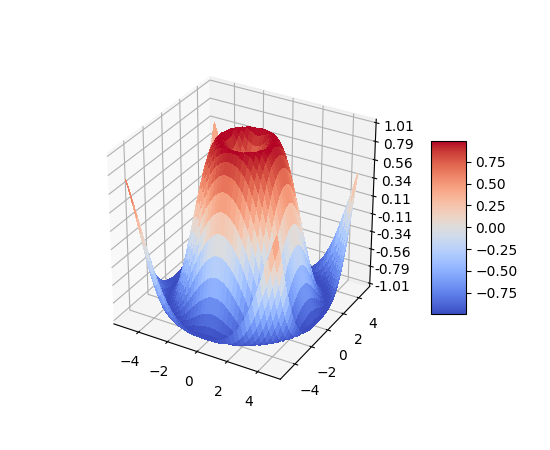
\includegraphics[width=0.25\textwidth]{surface3d_demo4}
    \caption{a nice plot}
    \label{fig:mesh1}
\end{figure}
 
As you can see in the figure \ref{fig:mesh1}, the function grows near 0. Also, in the page \pageref{fig:mesh1} is the same example.

The table \ref{table:1} is an example of referenced \LaTeX elements.
 
%LaTeX Warning: `!h' float specifier changed to `!ht'.
%\begin{table}[h!]
\begin{table}[!ht]
\centering
\begin{tabular}{||c c c c||} 
 \hline
 Col1 & Col2 & Col2 & Col3 \\ [0.5ex] 
 \hline\hline
 1 & 6 & 87837 & 787 \\ 
 2 & 7 & 78 & 5415 \\
 3 & 545 & 778 & 7507 \\
 4 & 545 & 18744 & 7560 \\
 5 & 88 & 788 & 6344 \\ [1ex] 
 \hline
\end{tabular}
\caption{Table to test captions and labels}
\label{table:1}
\end{table}

\section{Aufgabenstellung [todo]}

\section{Motivation [todo]}

\section{Zielsetzung [todo]}

\section{Gliederung [todo]}

\section{???Problemstellung?? [todo]}

In der Zeit vor den Navigationsgeräten wurden auf deutschen Straßen noch regelmäßig faltbare Straßenkarten von den Beifahrern verwendet um den Fahrer den Weg zu weisen. Bevor eine Straßenkarten verwendet werden kann, muss diese Erstellt werden. Dieser Prozess ist unter dem Begriff Kartenerstellung (engl. Mapping) bekannt. Der Detailgrad hängt dabei stark vom Verwendungszweck ab. Der erste Schritt nach dem entfalten der Straßenkarten bestand in der Lokalisierung (engl. Localization), also der Bestimmung der ungefähren Fahrzeugposition und dem Ziel der Reise auf der Straßenkarte. Darauf aufbauend wurde vom Beifahrer dann eine Route zwischen der aktuellen Fahrzeugposition und dem Ziel geplant und während der Fahrt weiter verfolgt, was auch als Pfad-Planung (engl. Path-Planning) bekannt ist.

Genauso wie der menschliche Agent muss auch jeder mobile Roboter für sich diese grundlegende Frage beantworten können. \glqq Wo bin ich?\grqq{}, \glqq Wo bin ich bereits gewesen?\grqq, \glqq Wohin gehe ich?\grqq{} und \glqq Welcher ist der beste Weg dahin?\grqq{}\cite{murphy2000introduction}.

Außerhalb von geschlossenen Räumlichkeiten (engl. Outdoor) erfolgt die Lokalisierung in der Regel mittels GPS, unter der Voraussetzung das eine ungehinderte Verbindung zu den GPS-Satelliten möglich ist. Die Lokalisierung ist in diesem Fall sehr einfach, da die GPS Koordinaten eindeutig sind und das Kartenmaterial bereits im gleichen Koordinatensystem vorliegt.

Innerhalb geschlossener Räumlichkeiten (engl. Indoor), wie in öffentlichen Gebäuden, Logistikhallen oder auch in Bergwerken, ist eine Lokalisierung mittels GPS nicht mehr möglich. Erschwerend kommt dazu, dass es in der Regel zu diesen Räumlichkeiten keine öffentlich verfügbaren Karten gibt oder diese sich wie im letzten Beispiel häufig ändern. Aus diesem Problemfeld haben sich Algorithmen für die Simultane Lokalisierung und Kartenerstellen (engl. Simultaneous Localization and Mapping (SLAM)) entwickelt.

Häufig werden SLAM Algorithmen verwendet um aus Kamerabildern oder \SI{360}{\degree} Abstandsmessungen eine Karte der Umgebung zu erstellen und sich in der gleichen zu lokalisieren. Der Fokus dieser Arbeit liegt jedoch auf den reinen Entfernungsbasieren SLAM (engl. Range Only SLAM (RO--SLAM)) Algorithmen. Hierbei werden nur die Informationen der Eigenbewegung und die Entfernungen zu mehreren, vorher unbekannten, Basisstationen genutzt um sich selbst zu Lokalisieren und eine Karte mit den Positionen der Basisstationen zu erstellen.